% Generated figure: ../gen_v10/make_figures.py (fig_allsets) from out/qcore6_heldout/results.json (sets C, ABC, D, E, F)
% and out/qcore9_heldout/results.json (set 4 = D, legacy scoring). Replaces fig_allsets6.tex. Values: ../gen_v10/figdata.json.
\begin{figure}[t]
\centering
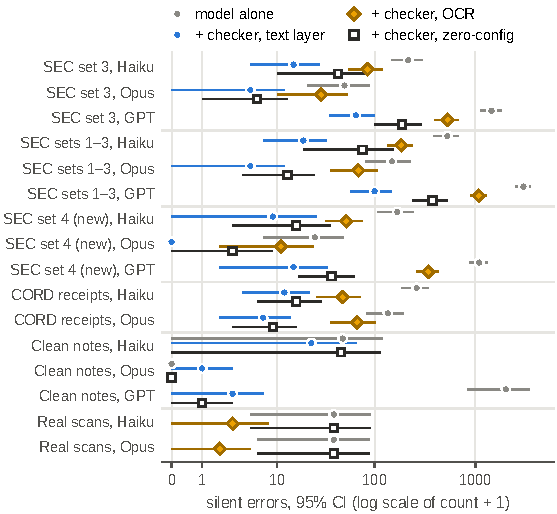
\includegraphics[width=\columnwidth]{v10_allsets.pdf}
\caption{Silent errors per held-out set and model, alone and with the checker (frozen \vq{6}; set~4: frozen \vq{9}), with 95\% bootstrap intervals; log axis of the count plus one, so 0 is the left edge. \emph{Text layer} and \emph{OCR} (docTR; real scans: the dataset's OCR) use hand identities; \emph{zero-config} uses none (real scans: no page text). With the text layer the checker cuts silent errors by one to two orders of magnitude; OCR cuts far less. Counts: Tables~\ref{tab:allsets} and~\ref{tab:d9}.}
\label{fig:allsets}
\end{figure}
